\chapter{Methodology, System Architecture and Experimentation Process}
\label{sec:method}

This chapter aims to clearly explain the research process used to analyze the problem and potential solutions.
Additionally it expands on the experimentation process undertaken in detail.

\section{Methodology}
A broad investigation --- in the form of a literature-review was undertaken --- to find, understand, compare and document the various cloud container platforms are currently available.
Additionally, interviews were performed at \emph{Allan Gray} focusing on tooling, architecture and deployment process utilized by the company.

\noindent \newline Each viable solution was then evaluated under the following four metrics:
Performance and Latency, Cost, Resilience, and Ease-of-Use.

\section{System Design and Architecture}

\begin{figure}[ht!]
  \centering
  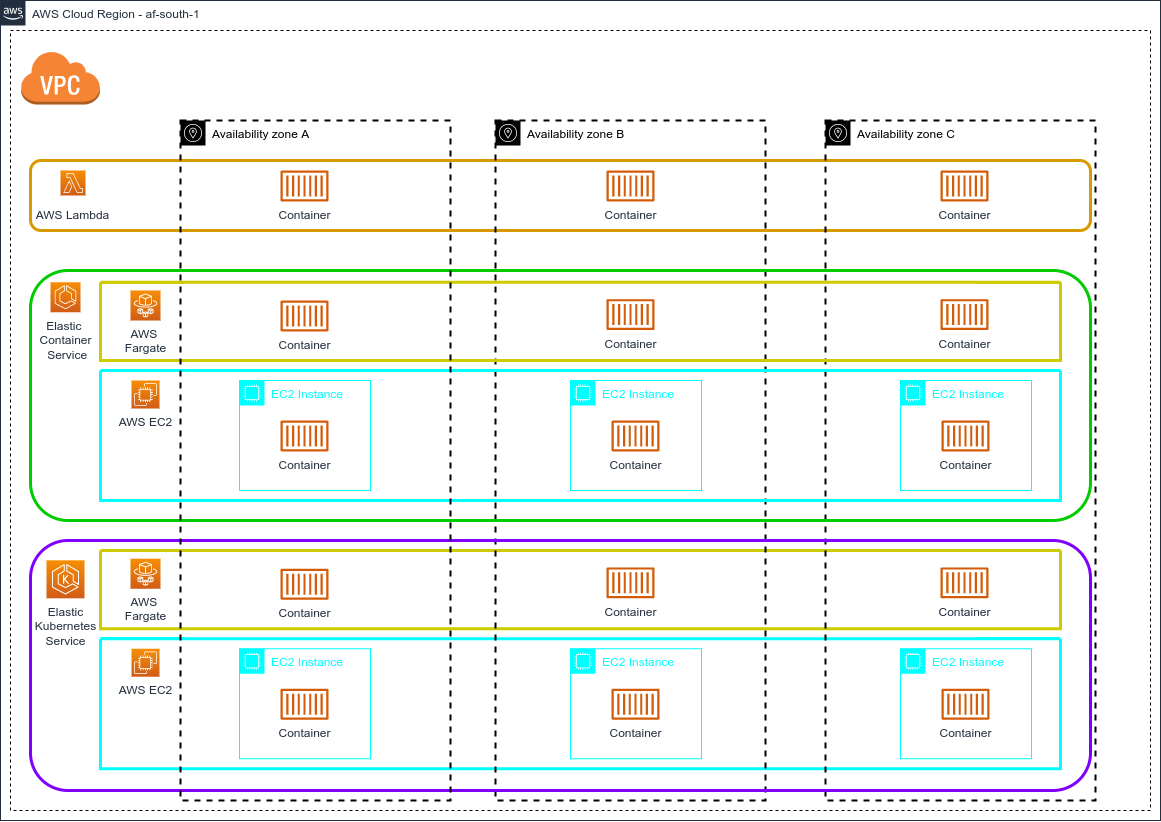
\includegraphics[width=\textwidth]{images/archDiagram.png}
  \caption{General Overview of System Architecture}
  \label{fig:archDiagram}
\end{figure}

As illustrated by Figure \ref{fig:archDiagram} each solution was evaluated in a controlled AWS \emph{VPC} in a single region (af-south-1), spread across three \emph{AZs} (where applicable).
Broad \textit{IAM} roles were created to grant required resources the correct permissions when accessing other resources.
An open \textit{SG} was attached to each resource to remove network restrictions as a potential block during testing.
The required cloud infrastructure was be deployed using \emph{Terraform} to ensure \emph{IaaC} principles are followed (and to maintain the \emph{correctness} of the testing environments).
Solutions which are not \emph{serverless} in nature were run on distinct dedicated isolated AWS EC2 instances of type \emph{m5.2xlarge}\cite{m5}, (each instance having 8 vCPU and 32GB of RAM). This ensured that each solution ran independently of one another.
Solutions which are serverless in nature automatically achieved the same goal.

Benchmark results of \emph{ephemeral} objects were written and stored on AWS \emph{S3} Buckets.

\emph{MSSQL} Databases were used as part of the application benchmark process, as this is the Database Engine of choice for \emph{Allan Gray}.
Existing on-premise instances were initially used as part of the the benchmarking process, however to remove network hops as a variable factor,
a distinct AWS \emph{RDS} \emph{MSSQL} Instance was created, with a new set of benchmark runs being performed.
Each solution targeted distinct tables so as to keep the environments distinct, even at a data level.

To create a baseline, all benchmarks were performed against an existing on-premise \emph{VMWare}\cite{vmware_2022} cloud of \emph{VM}s (each \textit{VM} running 8 vCPU and 24GB of RAM) running \emph{RKE} (\emph{Allan Gray}'s existing container-platform) \\

\noindent Required code to recreate the testing environment can be found as \emph{Terraform} code in the following GitHub repositories:
\begin{itemize}
      \item \emph{tool-deploy-eks}\cite{thameezb_2022} --- deploys an EKS cluster with all required dependencies
      \item \emph{tool-deploy-platform}\cite{thameezb} --- deploy an ECS cluster and all required dependencies, deploys benchmarking-suite, and tool-container-benchmark
\end{itemize}
\emph{Docker} image definitions can be found in Appendix \ref{appendix:docker_images}.
\emph{AMI} build-scripts can be found as \emph{packer} code in Appendix \ref{appendix:packer_ami_defintions}.
Additionally all other tooling or applications used can be found on GitHub\cite{bodhanya_2022}.

\section{Experimentation}
\subsection{Performance and Latency}
Performance and Latency were measured using two forms of benchmarking, the first following industry standard performance benchmarking using the phoronix-test-suite\cite{phoronix_test_suite} tool.
With the second being a custom-built application benchmark, which was able to focus on \emph{CRUD} based activities.
Each of these benchmarks were run at least three times, with the outputted results being averaged out.

\subsubsection{phoronix-test-suite}
The phoronix-test-suite is a high-customizable \emph{OSS} tool which acts as a wrapper to run various open-source benchmarking suites hosted by \emph{OpenBenchmarking.org}\cite{openbenchmarking.org_2020}.
A custom test-suite was created which targets specific aspects of a container-platform which is relevant to this project (and builds upon a previous testing methodology used by Potdar and Narayan\cite{POTDAR20201419}).
The selected tests are:
\begin{itemize}
  \item compress-7zip\cite{7zip_lzma_benchmark} --- runs a set of 7zip compressions and decompressions against a 10GB file using \emph{7zip}'s built in \emph{LZMA} benchmark.
        The benchmark primarily affects CPU and is measured in \emph{MIPS}.
  \item RAMspeed\cite{hollander_bolotoff_2002} --- performs four distinct floating-point memory intensive tasks (Add, Copy, Scale, and Triad) each measuring a different aspect of memory performance.
        The benchmark result is recorded as a measurement of speed (MB/S)
  \item mbw\cite{raas_2022} --- measures the amount of \textit{copy} memory bandwidth available to a user-application, simulating a generic user application 
        The benchmark result is recorded in terms of speed (MB/s)
  \item fs\_mark\cite{josefbacik_2014} --- evaluates a system's underlying file-system by performing heavily synchronous I/O tasks across multiple folders/drives
        Results are measured in terms of speed (number of files per second)
  \item m-queens\cite{sudden6_2014} --- solves the n-queens\cite{sloman_quanta} problem using multi-threading. Number of queens (n) was set to 18
        Results are measured in terms of time-to-completion (s).
\end{itemize}
In addition to the above, a \emph{sysbench}\cite{akopytov_2020} PrimeSieve benchmark was run for each solution (with max n=1000000), as an additional CPU specific benchmark.


The required tooling and configuration was then added to a Docker image built upon Ubuntu 20.04\cite{ubuntu_wiki}, which each solution then ran as a container.
Results were stored to \emph{S3}.

Tooling code is available on GitHub at\cite{tool_benchmarking_suite}.

\subsubsection{tool-container-benchmark}
\textit{tool-container-benchmark} is a custom built open-source benchmarking tool. This tool performs basic \emph{CRUD} operations against a Database of choice,
which mimics a portion of a typical enterprise workload. The tool starts of by clearing all projects in a specific table, creates a basic data-set within the table,
and performs a set of randomly chosen \textit{events} against a random project. An event is defined to be either a creation, update or delete operation.
The tool is written in \emph{go}\cite{go} and was natively compiled for the chosen container \emph{OS}. 

Allowed configuration:
\begin{itemize}
  \item Number of Events --- this allows a user to define how many events should be run per benchmark run
  \item Number of Projects --- this allows a user to define how many projects should be created per benchmark run (which creates an upper-bound of events per project)
  \item IsLambda --- this configures if the benchmark should run in a server or serverless mode
\end{itemize}

Tooling code is available on GitHub at\cite{tool_container_benchmark}.

\subsection{Cost}
Cost was measured in US Dollars using AWS's built in Cloud Cost Explorer tool\cite{blocher_juras_smith_2022}, with each system matched to cost using identification tags.
The total cost of running \textit{tool-container-benchmark} with \textit{30000} events (including all other required dependencies)
was measured per solution.
Additionally, a forecasted costing of running a long-lived service per solution (a single container which runs twenty-four hours a day for thirty days reserving .256 vCPU and 512MB of RAM)
was calculated using AWS's Pricing Calculator\cite{venning_2020} tool.

\subsection{Resilience and Reliability}
Resilience and Reliability were measured using \textit{TTR} when performing standard \textit{Chaos-Engineering} processes for container workloads.
These included evaluating the solution's ability to handle sudden scaling-in of container-workloads (that is to route network traffic to healthy replicas or respond to an unhealthy container by starting a new replica),
and actual deletion of container-workloads at a host level (that is stopping the container at a host-level and observing the solution's ability to recover) where possible.
Additionally an actual reboot of the underlying host (for \textit{Virtual Machine} based workloads) was also performed.
The \textit{SLA}'s and underlying architecture would also be taken into consideration when discussing this aspect.

\subsection{Ease-of-Use}
Ease-of-Use (being a highly subjective metric) was evaluated in terms of complexity to configure the solution environment, additional tooling required to deploy to said environment,
and finally the amount of changes required to deploy a container workload using this solution, with unit \textit{time} being the unit of comparison.
